\cotefile{37}
\scanpage{39}
\margin{\handwritten{SGA 4 \uline{VIII}}}

10. \uline{Compléments}: \uline{espaces algébriques et étendues algébriques}.

Nous donnons sous forme d'exercices quelques compléments, qui ne seront pas utilisés dans la suite du Séminaire.

10.1. Soit $(X,\underline{O}_X)$ un schéma, \deleted{notons par posons $X_{\mathrm{ét}}=\operatorname{Top}(X)$, de} sorte que\deleted{\unsure{n}} $(X_{\mathrm{ét}}^{\handwritten{\sim}},\underline{O}_X)$ est un topos annelé. Montrer qu'on peut \unsure{réoonstruire|réconstruire} le schéma $X$ à isomorphique unique près, quand on connait le topos annelé $(X_{\mathrm{et}}^{\handwritten{\sim}},\underline{O}_X)$ à équivalence près. (Utiliser 6.1 pour \unsure{rédonstituer|réconstituer} \deleted{$\operatorname{Top}(X)$} le topos $\operatorname{Top}(X)=\operatorname{Ouv}(X_{\mathrm{ét}}^{\handwritten{\sim}})^{\handwritten{\sim}}$, puis utiliser IV 4.\handwritten{2}.\handwritten{3}.) Plus précisément, montrer que si $X,X'$ sont deux schémas, alors l'applic\deleted{\unsure{a}}ation naturelle
\[
\operatorname{Hom}(X,X')\handwritten{\longrightarrow}\operatorname{Homtoplocan}(X_{\mathrm{ét}}^{\handwritten{\sim}},X'_{\mathrm{ét}}{}^{\handwritten{\sim}})
\]
\margin{\handwritten{\unsure{$\chi$|$\times$}}}
(notations de IV \handwritten{11.}) induit une équivalence entre la catégorie discrète définie par l'ensemble $\operatorname{Hom}(X,X')$ et la catégorie \uuline{Homtoplocan}$(X_{\mathrm{ét}}^{\handwritten{\sim}},X'_{\mathrm{ét}}{}^{\handwritten{\sim}})$ (où pour simplifier on désigne par $X_{\mathrm{ét}}^{\handwritten{\sim}}$ le topos étale de $X$ considéré comme topos annelé). (Utiliser IV 4.\handwritten{2}.\handwritten{3}.\deleted{\unsure{et}}\handwritten{)}
\margin{\handwritten{\deleted{\unsure{etc.}}}}

10.2. Soit $(E,\underline{O}_E)$ un topos annelé. Montrer que les conditions suivantes sont équivalentes (comparer IV \handwritten{9.}):
\margin{\handwritten{$\times$}}

(i) Il existe une famille $(X_i)_{i\handwritten{\in}I}$ d'objets de $E$ couvrant l'objet final, et une famille $(X'_i)_{i\handwritten{\in}I}$ de schémas, tels que pour tout $i\handwritten{\in}I$, le topos annelé induit $E_{/X_i}$ soit équivalent à $X'_{i\,\mathrm{ét}}{}^{\handwritten{\sim}}$.

(ii) Comme (i), avec $I$ réduit à un élément.

(iii) Il existe un schéma $X_{\handwritten{0}}$, et une prérelation d'équivalence $\deleted{R}\handwritten{X_1}$ dans $X_{\handwritten{0}}$ au sens de la catégorie (Sch) des schémas \handwritten{,}\deleted{\handwritten{\illegible{2}}} telle que $R$ soit étale i.e. le morphisme $p_1:\deleted{R}\handwritten{X_1\to}X_{\handwritten{0}}$ est étale, et que le topos annelé $(E,\underline{O}_E)$ soit équivalent au topos annelé déduit par recollement du diagramme \inserted{\handwritten{\unsure{$\frac12$-simplicial|2-simplicial}}} de topos annelés \inserted{\handwritten{étales}} \handwritten{associé\deleted{\unsure{s}} au diagramme de schémas}
\diagram{\begin{tikzcd}[ampersand replacement=\&]
X_{\handwritten{2}}\arrow[r,shift left=1.2ex]\arrow[r]\arrow[r,shift right=1.2ex] \& X_{\handwritten{1}}\arrow[r,shift left=.6ex]\arrow[r,shift right=.6ex] \& X_{\handwritten{0}}
\end{tikzcd}}
% The five arrows of the diagram are handwritten.
% archive sheet number: 38
\scanpage{40}
\margin{\handwritten{\unsure{$\chi$|$\times$}}}
où $X_2=(X_1,p_2)\mathbin{\mathrm{x}}_{X_{\unsure{o|0}}}(X_1,p_1)$ (cf. IV \handwritten{9} pour le procédé de recollement de topos par données de descente).

Lorsque les conditions précédentes sont satisfaites, on dira que le topos annelé $(E,\underline{O}_E)$ est une \uline{étendue algébrique}\deleted{\unsure{.}} (comparer avec la notion d'étendue topologique IV \handwritten{9.}).
\margin{\handwritten{$\times$}}

10.3. Montrer qu'une étendue algébrique a suffisamment de points.

\margin{\handwritten{$\times$}}
\unsure{Une|Bne} étendue algébrique est \uline{localement} annelé\handwritten{e} (IV \handwritten{11.}), et si $E,E'$ sont deux étendues algébriques, la catégorie \uline{Homtoplocan}$(E,E')$ (IV \handwritten{11.}) est un groupoïde (toute flèche est inversible). (Procéder pour le premier point comme dans IV \handwritten{9.}; pour le deuxième, utiliser IV \hspace{2em}.)
\margin{\handwritten{$\times\quad\times$}}

10.4. \inserted{\handwritten{(Comparer \uline{IV} 9.\hspace{1em})}} Soit $E$ une étendue algébrique. Montrer que les conditions suivantes sont équivalentes:
\margin{\handwritten{$\times$}}

(i) Pour toute étendue algébrique $E'$, la catégorie \deleted{Homtop} \uline{Homtoplocan}$(E',E)$ est rigide, i.e. \deleted{\unsure{c'est|est}} (comme c'est un groupoïde) elle est équivalente à une catégorie discrète.

(ii) Même énoncé, $E'$ étant le topos ponctuel annelé par un corps algébriquement clos.En d'autres termes, pour tout point géométrique (IV \handwritten{\unsure{11.|11b}}) de $E$, le groupe des automorphismes de $p$ est le groupe unité.
\margin{\handwritten{$\times$}}

(iii) (Lorsque $E$ est exprimé en termes d'une prérelation d'équivalence \inserted{étale} $X_1$ dans un schéma $X_o$, comme dans 10.2 (iii).) La prérelation d'équi\deleted{\unsure{k|r}}valence $(X_1,p_1,p_{2_{\deleted{\unsure{2}}}})$ dans le schéma $X_o$ est une relation d'équi\deleted{\unsure{k|r}}valence, i.e. le morphisme $(p_1,p_2):X_1\handwritten{\longrightarrow}X_o\mathbin{\mathrm{x}}X_o$ est un monomorp\deleted{\unsure{m|h}}hisme.

Lorsque ces conditions sont satisfaites, on dit que l'étendue algébrique $E$ est \uline{rigide}, ou encore que $E$ est un \uline{espace} \uline{algébrique} \handwritten{(*)}

\figure{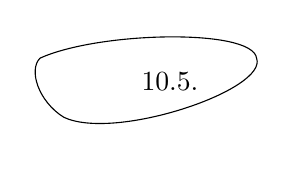
\begin{tikzpicture}
\node at (0,0) {10.5.};
\draw (-1.65,.30) .. controls (-.9,.64) and (1.05,.68) .. (1.10,.30) .. controls (1.25,-.10) and (-.70,-.76) .. (-1.35,-.45) .. controls (-1.67,-.25) and (-1.80,.15) .. (-1.65,.30);
\end{tikzpicture}}

\handwritten{(*) La terminologie est due à M. ARTIN, qui a mis en évidence l'importance de cette notion en Géométrie Algébrique.}
% archive sheet number: 39
\scanpage{41}
\figure{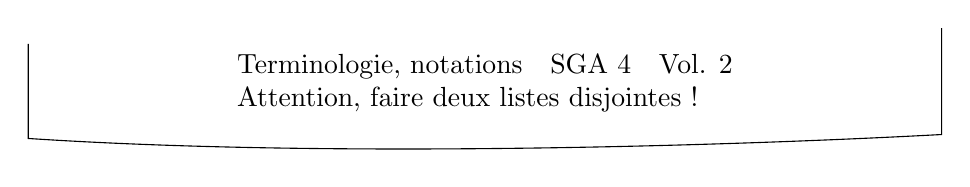
\begin{tikzpicture}
\node[align=left] at (0,0) {\handwritten{Terminologie, notations\quad SGA 4\quad Vol. 2}\\\handwritten{Attention, faire \uline{deux} listes disjointes !}};
\draw (-5.8,.5)--(-5.8,-.7) .. controls (-2,-.95) and (3,-.8) .. (5.8,-.65)--(5.8,.7);
\end{tikzpicture}}

\figure{\begin{tikzpicture}
\node[align=left] at (0,0) {(Sch)\qquad VII 1.1\\$\operatorname{Et}_{/X}\handwritten{,}\ X_{\mathrm{ét}}$\quad VII 1.2};
\draw (0,0) ellipse (2.8cm and .8cm);
\end{tikzpicture}}

Topologie étale (sur (Sch), sur un schéma)\quad étale topology (on (Sch), \inserted{on a scheme)}\handwritten{)}\quad VII 1.2

site étale d'un schéma\quad étale site of a scheme\quad VII 1.2

topos étale d'un schéma\quad étale topos of a scheme\quad VII 1.2

\figure{\begin{tikzpicture}
\node at (0,0) {$f_{\mathrm{ét}}$\qquad VII \unsure{1.4|1.1.4}};
\draw[line width=.8pt] (.65,.08)--(.78,.30);
\draw (0,0) ellipse (2.6cm and .4cm);
\end{tikzpicture}}
% A handwritten dark correction overlaps the middle of the f_et reference.

point géométrique d'un schéma\quad geometric point of a scheme\quad VIII 3.1.

foncteur fibre (relatif à un point géométrique d'un schéma)\quad fiber functor\deleted{\unsure{s}} (corresponding to a geometric point of a scheme)\quad VIII 3.3

\figure{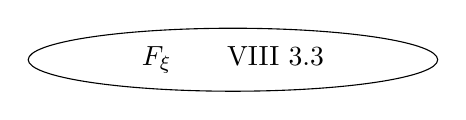
\begin{tikzpicture}
\node at (0,0) {$F_{\handwritten{\xi}}$\qquad VIII 3.3};
\draw (0,0) ellipse (2.6cm and .4cm);
\end{tikzpicture}}

hensélien (anneau local - )\quad henselian local ring\quad VIII 4.1

\deleted{Clôture} \unsure{hensélisé}\deleted{\unsure{enne|en}} d'un anneau local\quad henselization of a local ring\quad VIII 4.1

strictement local (anneau)\quad strictly local ring\quad VIII 4.2

\handwritten{---} id \handwritten{---} (schéma)\quad strictly local scheme\quad VIII 4.2

anneau \deleted{\unsure{à}}strictement local (d'un schéma en un point géométrique)\quad strictly local ring (of a scheme \unsure{àt|at} a geometric point)\quad VIII 4.3

hensélisé strict d'un anneau local\quad strict hens\deleted{\unsure{\'{}}}elisation of a local ring\quad VIII 4.4

localisé strict d'un schéma en un point géométrique\quad strict localization of a scheme at a geometric point\quad VIII 4.3

flèche de spécialisation\quad speciali\deleted{\unsure{s}}zation \deleted{\unsure{morphism}}\inserted{arrow}\quad VIII 7.2

spécialisation d'un point géométrique\quad specialization of a geometric \unsure{point}\quad VIII 7.2

générisation d'un point géométrique\quad generization of a geometric point\quad VIII 7.2

\figure{\begin{tikzpicture}
\node at (0,0) {$\handwritten{\overline}{X}(\handwritten{\xi})$};
\draw[rotate=35] (0,0) ellipse (.65cm and .4cm);
\node[anchor=west] at (.8,0) {($\handwritten{\xi}$ point géométrique du schéma $X$)\quad VIII 7.1};
\end{tikzpicture}}

Homomorphisme de spécialisation\quad \deleted{\unsure{f|t}} specialization homomorphism\quad VIII 7.7

\figure{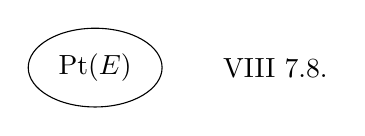
\begin{tikzpicture}
\node at (0,0) {\uline{Pt}$(E)$};
\draw (0,0) ellipse (.85cm and .5cm);
\node[anchor=west] at (1.5,0) {VIII 7.8.};
\end{tikzpicture}}
% archive sheet number: 40
\scanpage{42}
% The four front-surface entries are upside down in the supplied scan; read after a 180-degree rotation.
% Faint mirror-image text is show-through from the other face (scan 41), not a second inscription on this face.

(Sch)\qquad VII 1.1

\margin{\unsure{-}}
topologie étale (d'un schéma)\quad étale topology (of a\unsure{)} scheme)

topos étale (d'un schéma)\quad étale topos (of a scheme)

site étale d'un schéma\quad étale site of a scheme
% archive sheet number: 41
\scanpage{43}
suite spectrale de descente\quad spectral sequence of descent\quad VIII 8.1\quad XVII ....
\margin{\handwritten{*}}

Hochschild-Serre (suite spectrale de - )\quad VIII 8.4

\inserted{faisceau de torsion}\quad \inserted{torsion sheaf}

faisceau de p-torsion,\quad p-torsion sheaf,\quad IX 1.1

\figure{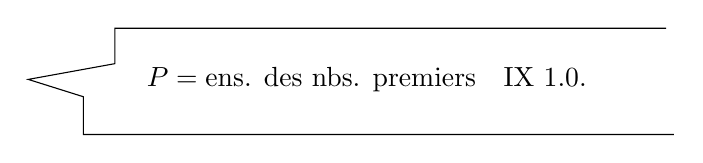
\begin{tikzpicture}
\node[align=left] at (0,0) {\handwritten{$\mathbb{P}={}$ens. des nbs. premiers\quad IX 1.0.}};
\draw (3.8,.65)--(-3.2,.65)--(-3.2,.2)--(-4.3,0)--(-3.6,-.22)--(-3.6,-.7)--(3.9,-.7);
\end{tikzpicture}}

faisceau de ind-p-groupes, faisceau de groupes ind-finis\quad sheaf of ind-p-groups, sheaf of ind-finite groups\quad \unsure{IX|YX} 1.5

localement constant (faisceau - )\quad locally constant sheaf\quad IX 2.0

constructible (faisceau d'ensembles, de groupes, de modules - )\quad constructible \deleted{\unsure{(}} sheaf of sets, groups or modules\deleted{)}\quad IX 2.3

connexe par arcs (schéma - )\quad arcwise connected scheme\quad IX 2.12

Kummer (théorie de - )\quad IX 3.2

\figure{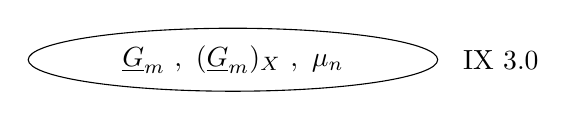
\begin{tikzpicture}
\node at (0,0) {$\underline{G}_m\ ,\ (\underline{G}_m)_X\ ,\ \handwritten{\mathbb{\mu}}_n$};
\draw (0,0) ellipse (2.6cm and .4cm);
\node[anchor=west] at (2.8,0) {IX 3.0};
\end{tikzpicture}}

Hilbert (théorème 90 de - )\quad IX 3.3

diviseur de Cartier\quad Cartier divisor\quad IX 3.4

Artin-Schreier (théorie de - )\quad IX 3.5

\figure{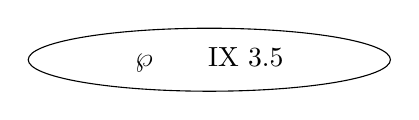
\begin{tikzpicture}
\node at (0,0) {$\handwritten{\wp}$\qquad IX 3.5};
\draw (0,0) ellipse (2.3cm and .4cm);
\end{tikzpicture}}

fa\deleted{\unsure{s}}i\deleted{\unsure{i}}sceau gratte-ciel\quad skyscraper sheaf\quad IX 4.1

morphisme trace\quad trace morphism\quad VIII 5.1 , XVII ...
\margin{\handwritten{*}}

$\handwritten{\ell}$-dimension cohomologique \inserted{d'un schéma}\quad $\handwritten{\ell}$-cohomological dimension \inserted{of a scheme}\quad X 1
\margin{\handwritten{$\ell$}}

\figure{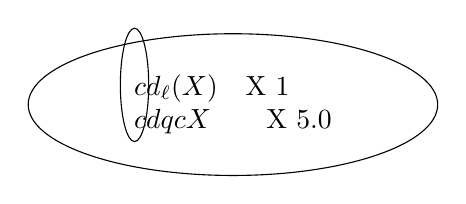
\begin{tikzpicture}
\node[align=left] at (0,0) {$\operatorname{cd}_{\handwritten{\ell}}(X)$\quad X 1\\$\operatorname{cdqc}X$\qquad X 5.0};
\draw (0,0) ellipse (2.6cm and .9cm);
\draw (-1.25,.25) ellipse (.18cm and .72cm);
\end{tikzpicture}}
\margin{\handwritten{$\ell$}}

fibration élémentaire\quad elementary fibration\quad XI 3.1

bon voisin\deleted{\unsure{g}}age (relativement à $S$)\quad nice neighbour\deleted{\unsure{h}}hood relative to $S$\quad \inserted{XI 3.2}

théorème de comparaison\quad comparison theorem\quad XI 4.4

\figure{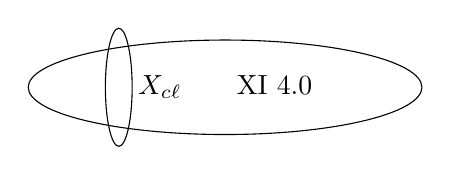
\begin{tikzpicture}
\node at (0,0) {$X_{c\handwritten{\ell}}$\qquad XI 4.0};
\draw (0,0) ellipse (2.5cm and .6cm);
\draw (-1.35,0) ellipse (.17cm and .75cm);
\end{tikzpicture}}

\figure{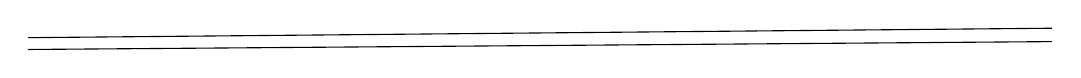
\begin{tikzpicture}\draw (0,0)--(13,.12);\draw (0,-.15)--(13,-.05);\end{tikzpicture}}
\margin{\handwritten{\uline{Vol. 2}}}

théorème de changement de base propre\quad proper base change theorem\quad XII 5.1

morphisme de changement de base\quad base change morphism\quad XII 4 , XVIII ...
\margin{\handwritten{*}}
% archive sheet number: 42
\scanpage{44}
\margin{\handwritten{\deleted{\unsure{XVI}} 5.2}}
\figure{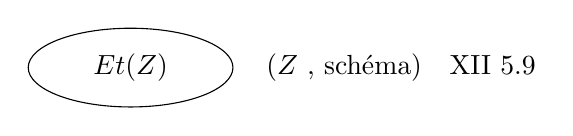
\begin{tikzpicture}
\node at (0,0) {$\operatorname{Et}(Z)$};\draw (0,0) ellipse (1.3cm and .5cm);
\node[anchor=west] at (1.6,0) {($Z$ , schéma)\quad XII 5.9};
\end{tikzpicture}}

Chow (lemme de - )\quad Chow lemma\quad XII 7.1

\deleted{Lemme de Chow}

Théorème de finitude \deleted{pour un morphisme propre\quad finiteness \unsure{theorm|theorem} for}\inserted{finiteness theorem}\quad \handwritten{$\overline{\underline{\mathrm{XIV}}}$ 1.1, \deleted{\unsure{XVI 5.1}}\inserted{$\overline{\underline{\mathrm{XVI}}}$ 5.1, 5.2} XVII ...) \inserted{$\overline{\underline{\mathrm{XIX}}}$ 5.1}}

\deleted{\handwritten{a)} pour morphisme propre\quad XIV 1.1}

\deleted{proper morphism\quad XIV 1.1}

\deleted{\handwritten{b)} pour $R^i_{\handwritten{!}}f$\quad XVII ...}
\margin{\handwritten{$\times$}}

\deleted{\handwritten{c)} pour un morphisme de type fini de schéma excellents\quad XIX 5.1}

\figure{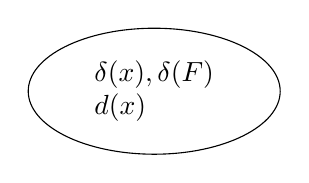
\begin{tikzpicture}
\node[align=left] at (0,0) {\inserted{\handwritten{$\delta(x),\delta(F)$}}\\$d(x)$};
\draw (0,0) ellipse (1.6cm and .8cm);
\end{tikzpicture}}
($x$, point d'un schéma\deleted{)}, \inserted{$F$ faisceau \deleted{sur $X$}}\handwritten{)}\quad \deleted{XIV (2.1)}\quad XIV 2

\inserted{\handwritten{Lefschetz}} \handwritten{(}théorème de \deleted{Lefschetz} affine\handwritten{)}\quad affine Lefschetz theorem\quad XIV 3.1 \handwritten{, XIX 6.1}

Morphisme \inserted{(universellement)} $n$-acyclique ($n$, entier)\quad \inserted{(universally)} $n$-acyclic morphisme\quad XV 1.3, 1.7

\deleted{Morphisme universellement $n$-acyclique\quad universally acyclic morphism}

\margin{\figure{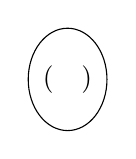
\begin{tikzpicture}\node at (0,0) {(\quad)};\draw (0,0) ellipse (.5cm and .65cm);\end{tikzpicture}}}
morphisme \inserted{(universellement\deleted{\unsure{à}})} 1-asphérique\quad \deleted{(universally)}\inserted{(universally) 1-aspheric} morphism\quad XV 1.7

\deleted{morphisme universellement 1-asphérique\quad universally 1-aspheric morphism}

Morphisme \inserted{(universellement)} localement $n$-acyclique\quad \inserted{(universally)} locally $n$-acyclic morphism\quad XV 1.11

morphisme \inserted{(universellement)} localement 1-asphérique\quad \inserted{(universally)} locally \deleted{\unsure{1}}\handwritten{1}-aspheric morphism\quad XV 1.11

\figure{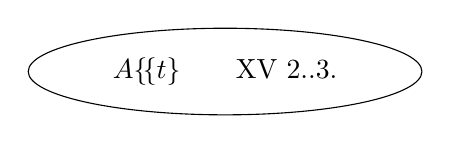
\begin{tikzpicture}
\node at (0,0) {$A\handwritten{\{\!\{}t\handwritten{\}}$\qquad XV 2\deleted{\unsure{.}}.3.};
\draw (0,0) ellipse (2.5cm and .55cm);
\end{tikzpicture}}

théorème de changement de base par morphisme lisse\quad base change theorem \deleted{for} \unsure{for|bor} smooth base change\quad XVI 1.2

théorème de spécialisation pour la cohomologie\quad speciali\deleted{\unsure{s}}zation theorem for cohomology\quad XVI 2.2

théorème de pureté cohomologique relatif\quad relative purity theorem for cohomology\quad XVI 3.6, \inserted{3.7}

théorème de pureté cohomologique absolue\quad absolute purity theorem for cohomology\quad XVI 3.9,XIX \inserted{1.2,2.1,3.2}

couple lisse \inserted{de schémas relatifs}\quad smooth pair of relative schemes\quad XVI 3.1

\deleted{Lemme} Abhyankar (lemme d'\deleted{\unsure{A}} - relatif )\quad relative \unsure{Anhyankar|Abhyankar}'s lemma\quad XVI 3.5

théorème de comparaison pour les schémas algébriques sur $\underline{C}$\quad comparison theorem for algebraic schemes over $\underline{C}$\quad XVI 4.1
% archive sheet number: 43
\scanpage{45}
\deleted{théorème de finitude}

théorème d'acyclicité locale\quad local acyclicity theorem\quad XV 2.1, XIX 4.1

couple régulier de schémas\quad regular pair of schemes\quad XIX 3.1

théorème de changement de base par morphisme régulier\quad base change theorem for regular base change morphism\deleted{e}\quad XIX 4.2

\figure{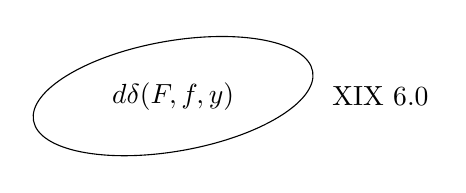
\begin{tikzpicture}
\node at (0,0) {$\deleted{\unsure{d}}\handwritten{\delta}(F,f,y)$};
\draw[rotate=10] (0,0) ellipse (1.8cm and .7cm);
\node[anchor=west] at (1.9,0) {XIX 6.0};
\end{tikzpicture}}

formellement séparable (k-algèbre - )\quad formally separable \inserted{\handwritten{k-}}algebra\quad XIX 6.7.\inserted{\handwritten{0}}

\figure{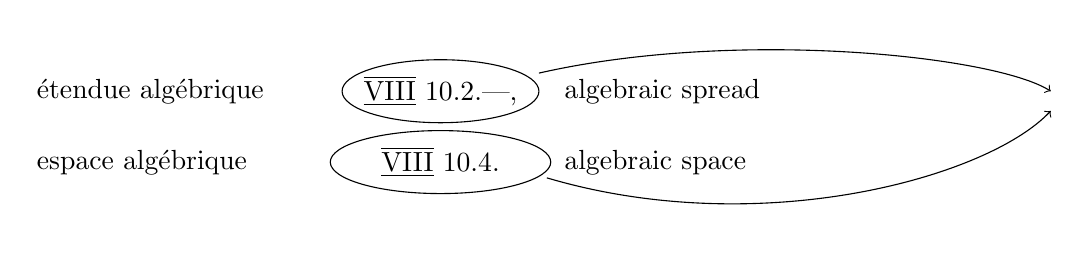
\begin{tikzpicture}
\node[anchor=west] at (0,0) {\handwritten{étendue algébrique}};
\node at (5.25,0) {\handwritten{$\overline{\underline{\mathrm{VIII}}}$ 10.2\unsure{.|,}}};
\node[anchor=west] at (6.7,0) {\handwritten{algebraic spread}};
\node[anchor=west] at (0,-.9) {\handwritten{espace algébrique}};
\node at (5.25,-.9) {\handwritten{$\overline{\underline{\mathrm{VIII}}}$ 10.4.}};
\node[anchor=west] at (6.7,-.9) {\handwritten{algebraic space}};
\draw (5.25,0) ellipse (1.25cm and .4cm);
\draw (5.25,-.9) ellipse (1.4cm and .4cm);
\draw[->] (6.5,.23) .. controls (9,.8) and (12.3,.45) .. (13,0);
\draw[->] (6.6,-1.1) .. controls (9.3,-1.9) and (12.2,-1.1) .. (13,-.25);
\end{tikzpicture}}
% archive sheet number: 44
\scanpage{66}
\begin{center}Commentaires Exp. X\end{center}

p.1, li.3 : référence pour $K.(X)$ : (IV 2.2 et 2.4).

p.1, li.15 : non nulle (sans trait d'union).

p.2, li.3 : référer à (EGA IV 3.1.4) pour le fait que $\operatorname{long}(\underline{F}_x)$ est finie.

p.2, li.8 : Prouver l'assertion ``Evidemment $K'$ contient ...'', il y a une petite suite exacte à écrire.

p.2, li.7 du bas : ``On sait (IV 2.11.1) ... ''

p.3, li.5 : (IV 1.4.1 et 2.11.1).

\deleted{p.3, li.\unsure{7|8}}

p.3, li.13 : \deleted{référence pour $K$} ajouter ``,noté $K^{\bullet}(X)_{\text{naïf}}$ dans (IV 2.2).''

p.3, li.14 : \deleted{\unsure{(VI|(IV}} (VI 3.2) si $X$ est quasi-compact, sinon ?

p.3 : Vider (1.2.1) et (1.2.2).

p.3, li.4 du bas : ``Rappelons (V 3.10) ...''

p.4, li. 3 : ``On a démontré (loc. cit.) ...''

p.4, li.9 : ``Rappelons (IV 2.10) ...''

p.4, li.8 du bas : numérotation canulée pour le Cor. 1.3.3. Peut-être vaut-il mieux , dans l'énoncé de ce corollaire, remplacer $X$ par \inserted{une autre lettre, $Z$ par exemple,} ce qui permettrait de préciser à la ligne du bas : ``tout sous-schéma intègre fermé $Z$ de $X$ ...''

p.5, li.4 : ``Pour \deleted{\unsure{éviter}} éviter toute confusion,...''

p.5, li.6 : (IV 2.11.1.2) .

p.5, li. 8 : référence \inserted{\handwritten{(V ...)}} pour $\handwritten{\alpha}^{\deleted{\unsure{i|x}}}(x)\handwritten{\in}\operatorname{Filt}^{i}(Z)$ .

p.6, li.1 : (V 3.11 (ii)) .

p.6, li. 6 du bas : ``on peut trouver (cf. VI 4.1) ...''

p.8, li. 1 et 2 du bas : références pour ``universellement caténaire'' et ``Cohen-Macaulay'' ((EGA IV 5.6.3), (EGA IV 5.7.1)). \handwritten{\deleted{\unsure{Voir}}}

\handwritten{référence pour l'assertion entre parenthèses \deleted{\unsure{:|?}} (EGA $\overline{\underline{\mathrm{IV}}}$ 6.3.7)}
% staple traces at upper left
% archive sheet number: 65
\scanpage{67}
\mspage{\handwritten{- 2 -}}

p.9, li. 2 du bas : qu'est-ce que désigne $e$ ?

p.10, li.7 : ``biéquidimensionnel (EGA $\unsure{0|O}_{\mathrm{IV}}$ 14.3.3).''

p.10, li. du bas : donner peut-être l'exemple de la fonction de dimension définie par un complexe dualisant (\handwritten{[}H\handwritten{]} V 7.1).

p.12, li. 7 du bas : ``telle que $G'$ soit ... soit ...''

p.13, li.11 du bas : ``continu pour la topologie ...''

p.14, li.12 : supprimer ``inversibles de $A$ de la forme''.

p.16; li. 3 : ``l'application composée ...''

p.16, li.9 : supprimer ``tel que $\dim(\operatorname{Supp}(\underline{F}))=j$''. Dire ce qu'on entend par``polynôme numérique''.

p.17 : pour la \unsure{commutativité|commutativitê|commutativite} du diagramme du bas, référer aux formules de changement de base (IV \hspace{3em}) ; la notation $\underline{s}_y$ devrait être remplacée par $s_{y_K}$ , où $y_K$ désigne l'image inverse de $y$ sur $X_K$ .

p.19, li.13 du bas : (IV 2.12.1).

p.20, li.6 : remplacer ``dans la catégorie dérivée'' par (IV 2.12.4).

p.22, li.8 : ``polynôme de Snapper (2.3.2) ...''

p.22, dans la formule (4.3.5), ne faut-il pas plutôt lire
\[
\handwritten{\alpha}_1+\ldots+\handwritten{\alpha}_d\handwritten{\leq}d\quad ?
\]

\deleted{p.22, li.6 du bas}

p.22, li.8 du bas : vider ``$=(\hspace{3em})$'' ?

p.24, li.8 du bas : ``$\dim(X)=\dim(Y)=d$''.

p.25, li.6 : vider la phrase ``On appelle équivalence numérique ...'', et rédiger ainsi (4.5.1) : ``... si les homomorphismes $\operatorname{Gr}_i(X)\handwritten{\longrightarrow}\underline{Z}$ (resp. $\operatorname{Gr}^i(X)\handwritten{\longrightarrow}\underline{Z}$) qu'ils définissent via le produit d'intersection (4.1.1) coïncident.''

p.25, li. 3 du bas : ``\unsure{Dé|De} 2.4.4 '' et non ``\unsure{De|Re} 2.4.3 ''.

Suggestion aux \S\S\ 2 et 4 : ajouter en remarque (ou exercice) que
% archive sheet number: 66
\scanpage{68}
\mspage{\handwritten{- 3 -}}
2.3.1 et 4.3.1 pour $F$ parfait résultent de R-R quand on en dispose. Dire aussi un mot du degré d'un diviseur sur une courbe ?

p.26, li.2 : \deleted{vider ``quelconque''} remplacer ``annelé quelconque'' par ``commutativement annelé''.

p.27, li.9 : ``1.3.3'' et non ``1.2.3''.

p.27, li.5 du bas : dire ``passe au quotient par $\operatorname{Filt}^{2}(X)$ et induit ...''

p.29, li.4 : écrire plutôt $H^0(X,\underline{Z})$ \inserted{ou $\Gamma(\underline{Z}_X)$} au lieu de $\Gamma(\underline{Z})$.

p.30, li.2 : il est peut-être prudent de supposer $X$ localement annelé.

p.30 : bas de page illisible.

p.31, li.1 : dire :``étant donné $M=T(\underline{O}^{\underline{n}_1},\ldots,\underline{O}^{\underline{n}_r})$ et la représentation ...''

p.31, li.4 : pourquoi supposer $M$ libre ? dire simplement ``par recollement de $M$ sur des cartes ...'' ou ``de la façon suivante.'', ce qui est \deleted{peut-être} encore mieux.

p.31, li.7 : ``tel que l'on ait ...''.Référer peut-être à la thèse de Giraud.

p.31, li.12 : supprimer ``fait opérer ... et'' et ``ainsi''. Après (6.1.4), dire qu'on \deleted{retrouve} a $M=T(\underline{O}^{\underline{n}_1},\ldots,\underline{O}^{\underline{n}_r})$.(référence Giraud). Pour (6.1.5), supposer $M$ localement libre.

p.32, \deleted{dire qu'on a une injection canonique} énoncer 6.2.2 en disant que l'injection canonique $\underline{\operatorname{Der}}(\operatorname{Gl}(\underline{n}))\handwritten{\unsure{\lhook\joinrel\relbar|\subset|\longleftarrow}}\operatorname{Sl}(\underline{n})$ est un isomorphisme. \handwritten{N'y a-t-il pas une référence dans Bible ou EGA3 ?}

p.34, li.10 du bas : ``voisinage étale'' au lieu de ``voisinage fpqc''.

p.3\deleted{\unsure{4}}5, li.12 du bas : même remarque.

p.35, li.4 du bas : que signifie $\operatorname{Gl}(n)(U)$ ? (si cela désigne les points de $\operatorname{Gl}(n)$ à valeurs dans $U$, alors la phrase n'a pas de sens).
% archive sheet number: 67
